\subsection{Cryptographic Ciphers}\label{sec:cryptography_basics:ciphers}

A \textbf{cipher} is a set of logically related algorithms --- such as a pair of encryption and decryption algorithms --- typically denoted with $\phi$. Besides correctness, ciphers may possess the following properties:

\begin{itemize}
	\item \textbf{perfect secrecy}: an attacker, given any one ciphertext only, cannot derive additional knowledge about the corresponding plaintext --- even when knowing the probability distribution of plaintexts. In other words, a plaintext can be mapped to all ciphertexts with the same probability;
	\item \textbf{semantic security}: an attacker, given a ciphertext, can feasibly derive only negligible additional knowledge about the corresponding plaintext. In other words, a cipher achieves semantic security if an attacker cannot feasibly distinguish between two ciphertexts that correspond to two different plaintexts. Semantic security is related to perfect secrecy, although the former is a strong theoretical notion (difficult to achieve in practice), while the latter is a more practical concept that focuses on the computational feasibility of the attacker's ability to learn information about the plaintext from the ciphertext;
	\item \textbf{(non-)malleability}: the en/decryption of data is malleable if it is possible to transform a ciphertext into another ciphertext which decrypts to a related plaintext (note that malleability differs from translation). More formally, given a ciphertext $c$ corresponding to a plaintext $m$, it is possible to generate another ciphertext $c'$ which decrypts to $f(m)$ for a known function $f$ --- without necessarily knowing or learning $m$. Although malleability is generally an undesirable property, it is the basis for \gls{he};
	%TODO (\Cref{future_sec:advanced_cryptography:homomorphic_encryption});
\end{itemize}

Another property relevant to ciphers (but also to, e.g., hash functions as discussed in \Cref{sec:hash_functions}) is the avalanche effect. Briefly, the avalanche effect states that a tiny change in any of the inputs of an algorithm (e.g., a bit flips) should make the output change significantly (e.g., half the output bits flip). The lack of the avalanche effect implies poor randomization, hence vulnerability to cryptanalysis.

A cipher having the perfect secrecy property is usually called \textbf{perfect cipher}. A cipher is perfect if a key is not reused to encrypt different plaintexts; otherwise, Shannon's Theorem no longer guarantees perfect secrecy. 

\remarkBlock{The Clever Boy Assumption and the Shannon's Theorem}{The so-called \textbf{clever boy assumption} states that the choice of keys for a cipher is not influenced by the choice of plaintexts. In simpler words, plaintext and keys are independent --- a realistic assumption for (ideally) all scenarios. The clever boy assumption is a prerequisite for the \textbf{Shannon's Theorem}: assuming that the set of keys, plaintexts, and ciphertexts of a cipher $\phi$ are equal and comprise $n$-bit strings\footnote{The set of all $n$-bit strings is denoted as either $\mathbf{\{0, 1\}^n}$ or $\{\mathbb{F}_2\}^n$. For instance, $\mathbf{\{0, 1\}^3} = \{000, 001, 010,$ $011, 100, 101, 110, 111\}$} only --- formally, $\Keys = \Plaintexts = \Ciphertexts = \{0, 1\}^n$ --- Shannon's Theorem states that $\phi$ is a perfect cipher if and only if ($i$) the keys are perfectly random and ($ii$) there exists one key only mapping a given plaintext to a given ciphertext --- formally, $\exists! k \in \Keys : \phi_k(m) = c~\forall m \in \Plaintexts, c \in \Ciphertexts$.}

Note that, in a perfect cipher, there are as many keys as plaintexts and that, more importantly, keys have the same length as plaintexts. As a consequence, perfect ciphers cannot be broken even by brute force attacks (\Cref{sec:cryptographic_security_overview:attacks}). As said before, perfect secrecy is a strong theoretical notion difficult to achieve in practice. An example of a perfect cipher is the \textbf{one-time pad cipher} (also called \textit{Vernam cipher}) where ciphertexts are obtained by \texttt{xor}-ing the plaintext and the key. Unfortunately, perfect ciphers are not practical.

Besides keys, ciphers typically consider as input also \textbf{\glspl{iv}}. Essentially, an \gls{iv} is a (pseudo)random
%TODO (\Cref{future_sec:randomness})
sequence of bytes used as additional input to the algorithms of a cipher to achieve semantic security. More in detail, \glspl{iv} prevent patterns and repetitions in ciphertexts which may be exploited by attackers. \glspl{iv} are usually required to be random but not secret and, more importantly, must never be reused --- especially under the same cryptographic key. A sequence of all-zero bytes is usually not suitable as \gls{iv}. \glspl{iv} are also called \textit{starting variables}. Although having slightly different purposes and applications, \glspl{iv} are essentially equivalent to nonces and these two terms \textbf{are often used interchangeably} (a \textbf{nonce} is a number used just once in cryptographic protocols usually for preventing replay attacks --- see \Cref{sec:security_of_cryptographic_protocols}).

A cipher comprising algorithms operating on fixed-length blocks of data --- one block at a time --- is called \textbf{block cipher}. Conversely, a cipher comprising algorithms operating on one bit of data at a time is called \textbf{stream cipher}.

\paragraph*{Block Ciphers.} A block cipher is a (keyed pseudo)random permutation family on the mappings between plaintexts and ciphertexts (if a block cipher is a true random permutation, then it is a perfect cipher). Block ciphers are slower but deemed theoretically more secure than stream ciphers. Usually, block ciphers take as input a key which is reused on each block of data. An example of a well-known and widely used block cipher is \gls{aes} (\Cref{sec:symmetric_cryptography:ciphers}). 

\curiosityBlock{Do asymmetric ciphers qualify as block ciphers?}{Although it is true that asymmetric cryptography (\Cref{sec:asymmetric_cryptography}) usually operates on fixed-length blocks of data, asymmetric ciphers are not considered block ciphers, as they do not match the standard definition of the term --- that is, a (keyed pseudo)random permutation. Moreover, an asymmetric cipher should not be used over a piece of data larger than the size of the cipher's block; in case this happens, the use of hybrid cryptography is preferred (\Cref{sec:hybrid_cryptography}).}

Block ciphers have a \textbf{mode of operation} which specifies how to combine multiple blocks. The most common or known modes of operation are:

\begin{itemize}
	\item \textbf{\gls{ecb}}: each block of plaintext is encrypted into a corresponding block of ciphertext independently from other blocks. \gls{ecb} achieves high performance by allowing for parallel encryption and decryption and provides random read access (i.e., blocks can be decrypted independently). However, \gls{ecb} is deprecated because it lacks key diffusion --- that is, similar blocks of plaintext result in similar blocks of ciphertext --- and requires padding whenever the length of the plaintext is not (integral) multiple of the block size. Moreover, \gls{ecb} does not inherently provide integrity and preserves the structure of the plaintext in the ciphertext (as shown by the famous \gls{ecb} penguin image --- see \Cref{figure:ecb_penguin});
	\item \textbf{\gls{cbc}}: each block of plaintext is \texttt{xor}-ed with the previous block of ciphertext before encryption. \gls{cbc} provides random read access (i.e., blocks can be decrypted independently). However, it does not inherently provide integrity, may need padding, and prescribes sequential encryption --- hence, limiting parallel processing and worsening efficiency --- but allows parallel decryption;
	\item \textbf{\gls{cfb}}: each block of plaintext is \texttt{xor}-ed with the previous block of ciphertext to generate the next ciphertext block --- in a sense, \gls{cfb} converts a block cipher into a stream cipher. \gls{cfb} provides random read access (i.e., blocks can be decrypted independently) and does not require padding, but does not inherently provide integrity and prescribes sequential encryption --- hence, limiting parallel processing and worsening efficiency --- while still allowing parallel decryption;
	\item \textbf{\gls{ofb}}: the key is used to generate a sequence of bytes called \textbf{keystream} and then --- similarly to \gls{cfb} --- each block of plaintext is \texttt{xor}-ed with the keystream. In a sense, \gls{ofb} converts a block cipher into a stream cipher. \gls{ofb} does not require padding but does not provide random read access (i.e., blocks can be decrypted independently), does not inherently provide integrity, and prescribes sequential encryption and decryption --- hence, limiting parallel processing and worsening efficiency;
	\item \textbf{\gls{ctr}}: blocks of plaintext are numbered sequentially (usually by increments of 1), and the number is combined (e.g., summed or concatenated) with a (unique) counter --- that is, the \gls{iv} --- and then encrypted; the result of this encryption is \texttt{xor}-ed with the plaintext of the block to produce the corresponding ciphertext --- in a sense, \gls{ctr} converts a block cipher into a stream cipher. \gls{ctr} provides random read access (i.e., blocks can be decrypted independently), does not require padding, and achieves high performance by allowing for parallel encryption and decryption, but does not inherently provide integrity. \gls{ctr} is also called \textit{integer counter mode} and \textit{segmented integer counter};
	\item \textbf{\gls{gcm}}: one of the most used in 2025, provides both confidentiality and authenticity. \gls{gcm} is so called because it combines \gls{ctr} with the Galois mode for authenticity. Similarly to \gls{ctr}, in \gls{gcm} blocks are numbered sequentially (usually by increments of 1), and the number is combined (e.g., summed or concatenated) with a (unique) counter --- that is, the \gls{iv} --- and then encrypted; the result of this encryption is \texttt{xor}-ed with the plaintext of the block to produce the corresponding ciphertext --- in a sense, \gls{gcm} converts a block cipher into a stream cipher. The blocks of ciphertext are considered coefficients of a polynomial manipulated in the corresponding Galois field (see the concept of fields in \Cref{sec:mathematical_underpinnings:fields}). Finally, \gls{gcm} produces a tag providing authenticity. \gls{gcm} provides random read access (i.e., blocks can be decrypted independently), does not require padding, and achieves high performance by allowing for parallel encryption and decryption;
	\item other less commonly used modes of operation are \gls{ccm}, \gls{xts}, \gls{eax}, \gls{siv}, \gls{ocb}, and \gls{lrw}.
	\warningBlock{Which modes of operation (not) to use}{\gls{gcm} or \gls{ccm} are the preferred modes of operation: other common or known modes of operation are not as secure or efficient, and other less commonly used modes of operation may be complex to use or configure and may lack support by available implementations.}
\end{itemize}

\begin{figure}[t!]
	\begin{center}
		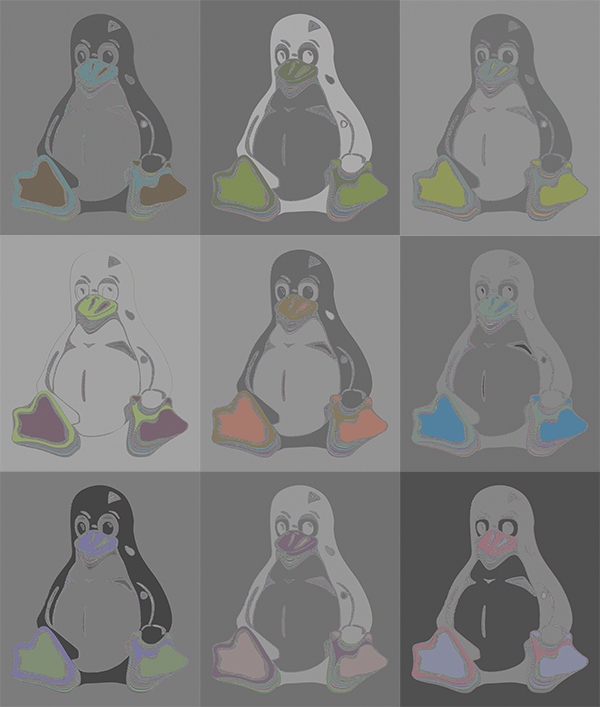
\includegraphics[width=0.5\linewidth]{resources/img/ecb_penguin.png}
		\caption{Multiple \gls{ecb} encryptions with the \gls{aes} symmetric block cipher (\Cref{sec:symmetric_cryptography:ciphers:aes}) of the Linux penguin mascot with different keys; as noticeable, the underlying image is clearly recognizable, even though ideally encrypted --- from \url{https://words.filippo.io/the-ecb-penguin/}.}
		\label{figure:ecb_penguin}
	\end{center}
\end{figure}

\paragraph*{Stream Ciphers.} Differently from block ciphers, stream ciphers are usually faster but deemed theoretically less secure than block ciphers. Usually, stream ciphers take as input a key that is --- often combined with an \gls{iv} and then --- used to generate an (ideally infinite pseudo)random keystream. Ultimately, the keystream is used for performing (several) bit-wise operations on the plaintext, hence obtaining the ciphertext
%TODO (\Cref{future_sec:randomness}
for more details on randomness in cryptography). An example of a well-known and widely used stream cipher is Salsa20/ChaCha20 (\Cref{sec:symmetric_cryptography:ciphers}). 
